\documentclass[a4paper]{scrartcl}
\usepackage[utf8]{inputenc}
% \usepackage{showframe} % disable this to hide #border.
\usepackage{wrapfig}
% Example:
% \begin{wrapfigure}{R}{0.4\textwidth}
% \centering
% 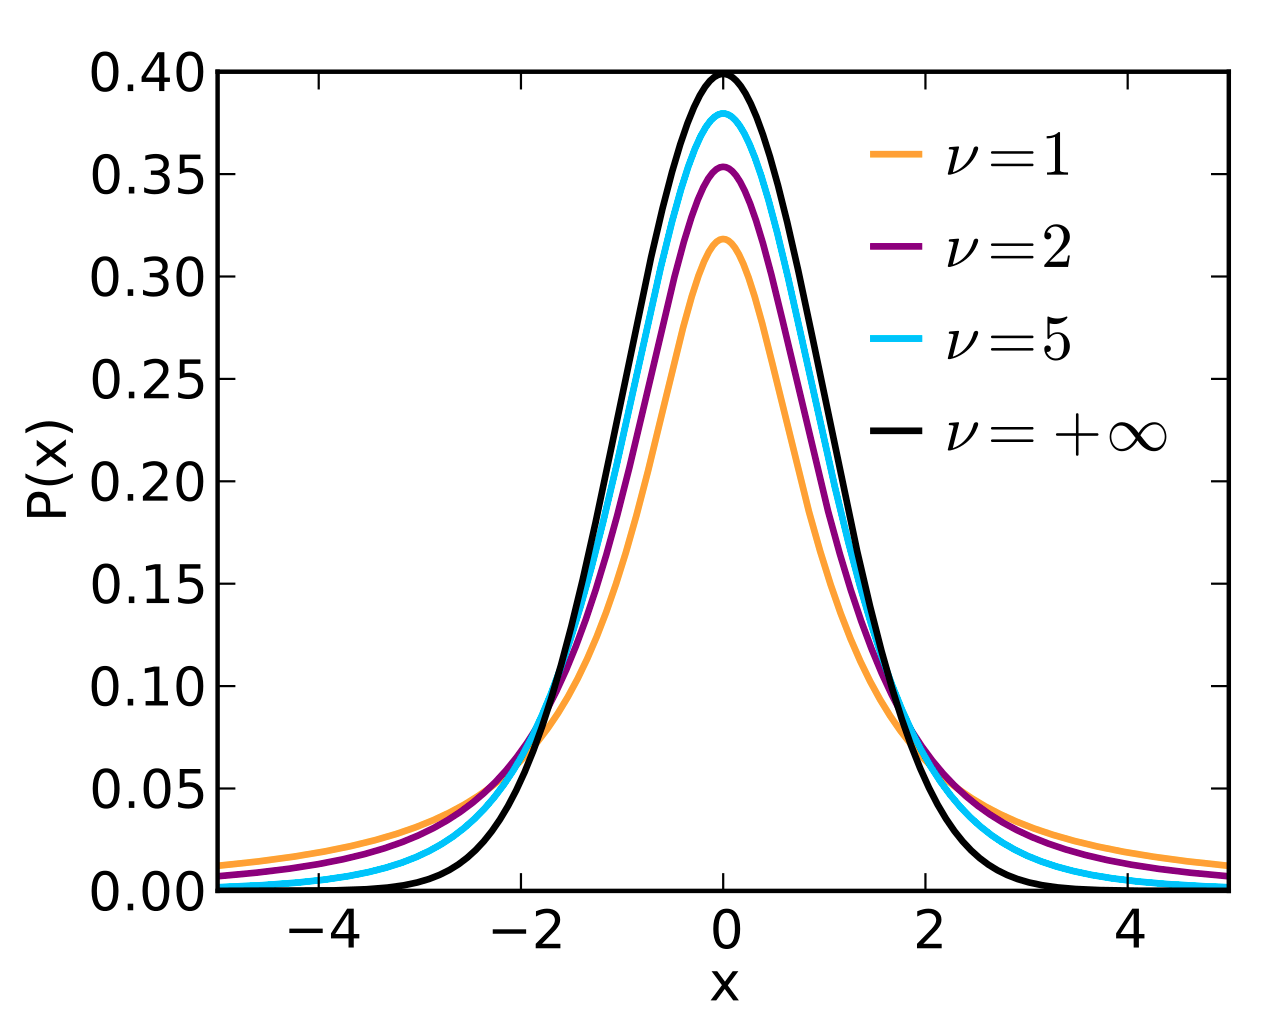
\includegraphics[width=0.35\textwidth]{assets/lectures_part_3-91d0349d.png}
% The PDF of the Student distribution.
% \end{wrapfigure}


\usepackage[english, russian, ukrainian]{babel}
\usepackage{misccorr,
            color,
            ragged2e,
            amsfonts,
            amsthm,
            graphicx,
            systeme,
            amsmath,
            mdframed,
            lipsum,
            mathtools,
            setspace
            }

\renewcommand\qedsymbol{$\blacksquare$}
\renewcommand*{\proofname}{\text{Доведення}}

\theoremstyle{definition}
\newtheorem*{defo}{Означення}
\newtheorem*{lemme}{Лема}
\newtheorem*{example}{Приклад}
\theoremstyle{remark}
\newtheorem*{remark}{Зауваження}
\theoremstyle{definition}
\newtheorem*{consequence}{Наслідок}
\theoremstyle{definition}
\newtheorem{statement}{Твердження}[section]
\newmdtheoremenv{boxteo}{Теорема}[section]

\setlength{\parindent}{0em}
\setlength{\parskip}{0.5em}
\DeclareMathOperator*\lowlim{\underline{lim}}
\DeclareMathOperator*\uplim{\overline{lim}}

\newcommand\independent{\protect\mathpalette{\protect\independenT}{\perp}}
\def\independenT#1#2{\mathrel{\rlap{$#1#2$}\mkern2mu{#1#2}}}

\usepackage{tikz}
\newcommand*\circled[1]{\tikz[baseline=(char.base)]{
  \node[shape=circle,draw,inner sep=1pt] (char) {#1};}}

% Default fixed font does not support bold face
\DeclareFixedFont{\ttb}{T1}{txtt}{bx}{n}{12} % for bold
\DeclareFixedFont{\ttm}{T1}{txtt}{m}{n}{12}  % for normal

% Custom colors
\definecolor{deepblue}{rgb}{0,0,0.5}
\definecolor{deepred}{rgb}{0.6,0,0}
\definecolor{deepgreen}{rgb}{0,0.5,0}

\usepackage{listings}

% Python style for highlighting
\newcommand\pythonstyle{\lstset{
language=Python,
basicstyle=\ttm,
morekeywords={self},              % Add keywords here
keywordstyle=\ttb\color{deepblue},
emph={MyClass,__init__},          % Custom highlighting
emphstyle=\ttb\color{deepred},    % Custom highlighting style
stringstyle=\color{deepgreen},
frame=tb,                         % Any extra options here
showstringspaces=false
}}


% Python environment
\lstnewenvironment{python}[1][]
{
\pythonstyle
\lstset{#1}
}
{}

% Python for external files
\newcommand\pythonexternal[2][]{{
\pythonstyle
\lstinputlisting[#1]{#2}}}

% Python for inline
\newcommand\pythoninline[1]{{\pythonstyle\lstinline!#1!}}

%                 USAGE:
% \begin{python}
% class MyClass(Yourclass):
%     def __init__(self, my, yours):
%         bla = '5 1 2 3 4'
%         print bla
% \end{python}
%
%
% \pythonexternal{demo.py}
%
%
% Definition \pythoninline{class MyClass} means \dots

\def\be{\begin{equation}}      % equation
\def\ee{\end{equation}}        % ...
\def\i{\infty}                 % infinity
\def\d{\partial}               % dx dy - partial     = \d
\def\bdash{\ \Big|\  }         % big vertical line   = |
\def\index{\mathbb{I}}         % indicator
\def\res#1{\underset{#1}{\mathrm{res}}}

\begin{document}
\tableofcontents
\newpage

\begin{center}
	\Huge \textbf{Лишки (вычеты)}
\end{center}
\par
\section{Означення.}
 $f(z)$ -- аналітична в околі т. $z_0$ за виключенням самої $z_0 : $$$\left\lbrace z \bdash 0 < \left| z - z_0 \right| < \delta \right\rbrace$$
  $\gamma $ -- контур, що охоплює $z_0$ та належить проколотому околу $z_0$. \par
  \textbf{Лишком} $f(z)$ в точці $z_0$ називають:
  $$
  \res{z=z_0} f(z) = \frac{1}{2 \pi}   \int\limits_{\gamma}^{}{f(z)\mathrm{d} z}
  $$
\begin{remark}
  З теореми Кошы для неоднозв'язної області випливає, що $\forall \gamma_1 , \gamma_2$, що охоплюють т. $z_0$ та належать $\left\lbrace z \bdash 0 < \left| z - z_0 \right| < \delta \right\rbrace$, виконується рівність:
  $$
  \int\limits_{\gamma_1}^{}{f(z)\mathrm{d} z}=
  \int\limits_{\gamma_2}^{}{f(z)\mathrm{d} z}
  $$
  Таким чином, $\res{z=z_0} f(z)$ не залежить від $\gamma$.
\end{remark}
\begin{boxteo}
 $f(x)$ -- аналітична в $\left\lbrace z \bdash 0 < \left| z - z_0 \right| < \delta \right\rbrace$. Тоді:
 $$
 \res{z=z_0} f(z) = C_{-1},
 $$
 де $C_{-1}$ -- коефіцієнт головної частини ряду Лорана при $ \frac{1}{z - z_0} $.
\end{boxteo}

\section{Методи знаходження лишків.}
\begin{lemme}
  $z_0$ -- \textit{усувна} особлива точка $f(z)$. Тоді:
  $$
  \res{z = z_0} f(z) = 0
  $$
\end{lemme}
\begin{lemme}
  $z_0$ -- \textit{суттєва} особлива точка. Тоді:
  \begin{center}
   $\res{z = z_0} f(z)$ рахується \textbf{тільки за розкладом} в ряд Лорана.
  \end{center}
\end{lemme}

\begin{lemme}
  $z_0$ -- \textit{полюс} порядка $k$. Тоді:
$$
\res{z=  z_0} f(z) = \frac{1}{(k-1)!}  \lim\limits_{z\to z_0}{ \left( f(z) * (z-z_0)^k \right)^{(k-1)}}
$$
\end{lemme}

\subsection{Часткові випадки.}
\begin{enumerate}
  \item $z_0$ - полюс першого порядку. Тоді:
  $$
  \res{z =  z_0} f(z) =  \lim\limits_{z\to  z_0}{ f(z) (z- z_0)} =
  $$
  \item $f(z) = \dfrac{\varphi(z)}{\psi(z)} $ така, що:
  $
  \varphi(z_0)  \neq  0 \quad \psi(z_0) = 0 \quad \psi'(z_0) \neq 0
  $.
  Тодi: $$ \res{z = z_0} f(z) = \frac{\varphi(z_0)}{
  \psi'(z_0)
  } $$
\end{enumerate}
\section{Нескінчена особлива точка. Ряд Лорана в околі $z = \infty$.}
Перетворення $\omega = \frac{1}{z} $ переводить $z = \infty$ в т. $\omega = 0$.\par
Розглядаємо: $ \omega  = \dfrac{1 }{z}   \ \Longleftrightarrow \ z = \dfrac{1}{\omega}   \quad
z_0 = \infty   \ \Longleftrightarrow \ \omega_0 = 0
  $.
  $$
  f(z) =  \cdots =  \underbrace{\sum\limits_{k = 1}^{ \infty}{C_{-k} z^k}}_{\text{головна}} + \underbrace{\sum\limits_{n = 0}^{ \infty}{ \frac{C_{n}}{z^n} }}_{\text{правильна}}
  $$

\textit{Коефіцієнт ряду} обчислюється за формулою:
$$
C_n = \frac{1}{ 2 \pi i}  \int\limits_{\gamma}^{}{f(z) z^{n-1}\mathrm{d} z}
$$

\begin{defo}
 Точка $z_0 = \infty $ є ізольованою, якщо:
 $$
 \exists R \ \forall z \in \left\lbrace  z  \bdash R < \left| z \right| \right\rbrace : f(z)  \text{ -- аналітична.}
 $$
\end{defo}
\newpage
\begin{defo}
 Точка $z_0 = \infty $ -- ізольована, називається:
 \begin{itemize}
   \item \textit{усувною}, якщо $ \exists  \lim\limits_{z\to  \infty}{f(z)} = A \pm \infty$.
   \item \textit{полюсом}, якщо $ \exists  \lim\limits_{z\to  \infty}{f(z)} = \infty$.
   \item \textit{суттєвою}, якщо $ \nexists  \lim\limits_{z\to  \infty}{f(z)}$.
 \end{itemize}
\end{defo}
Порядок полюса $z_0 = \infty$:
$$
 \lim\limits_{z\to  \infty}{ f(z)} = \infty \ \Longleftrightarrow \   \lim\limits_{z\to  \infty}{ \frac{1}{f(z)} } = 0
$$
Тодi порядок полюса  $z_0 = \infty$ є кратність нуля $z_0 = \infty$ для $h(z) = \dfrac{1}{f(z)} $


\subsection{Характеристика ізольованої особливої точки $z_0 = \infty$ за розкладом в ряд Лорана.}
\textbf{Твердження.} $z_0 = \infty$ -- ізольована, особлива точка для $f(z)$. Тоді:
\begin{enumerate}
  \item $z_0 = \infty$ -- \textit{усувна}: ряд Лорана не містить головної частини.
  \item $z_0 = \infty$ -- \textit{полюс} кр. k: ряд Лорана містить k доданків головної частини.
  \item $z_0 = \infty$ -- \textit{суттєва}: ряд Лорана містить безліч доданків головної частини.
\end{enumerate}
\begin{defo}
  $z_0$ -- ізольована особлива точка функції $f(z)$.\par
   \textbf{Лишком} функціі $f(z)$ в т. $z_0 = \infty$ називають:
   $$
   \res{z=\infty} f(z) = \frac{1}{2 \pi }  \int\limits_{\gamma^-}^{}{ f(z) \mathrm{d} z}
   $$
\end{defo}

\subsection{Пошук лишків. Зв'язок з рядом Лорана.}
 \begin{boxteo}
$z_0 = \infty$ -- ізольована, особлива точка для $f(z)$. Тоді:
$$
\res{z = z_0} f(z) = -C_1
$$
де $C_{1}$ -- коефіцієнт головної частини ряду Лорана $f(z)$ в околі $z_0 = \infty$, тобто коефіцієнт при доданку $ \frac{1}{z} $.
 \end{boxteo}
\begin{remark}
  Навіть у усувної точки $z_0 = \infty$ лишок може бути ненульовим.
\end{remark}
\newpage
\section{Застосування лишків для обчислення інтегралів.}
\begin{boxteo}[Коші, для лишків І]
  Задана $f(x)$ -- аналітична в області $D$ за вийнятком скінченої кількості особливих точок $z_1 , \dots , z_n$.\par
  $\gamma$ -- замкнений контур в $D$, який охоплює $z_1 , \dots , z_n$. Тоді:
  $$
   \int\limits_{\gamma}^{}{ f(z) \mathrm{d} z} = 2 \pi i  \sum\limits_{k = 1}^{n}{ \res{z = z_k }f(z)}
  $$
\end{boxteo}
\begin{boxteo}[Коші, для лишків II]
  Задана $f(x)$ -- аналітична в області $D$ за вийнятком скінченої кількості особливих точок $z_1 , \dots , z_n$. Тоді:
  $$
    \sum\limits_{k = 1}^{n}{\res{z = z_k }f(z) } + \res{z = \infty} f(z) = 0
  $$
\end{boxteo}
\begin{remark}
  Ми розглядаємо випадок скінченої кількості особливих точок, бо в випадку нескінченої кількості з'являється гранична точка(точки) із множини особливих, що не будуть ізольованими.
\end{remark}

\subsection{ Застосування теорії лишків для дійсних інтегралів.}

\textbf{I.} $R(x,y)$ --- дробово-раціональна функція від $x,y$:
$$
R(x,y) = \frac{P(x,y)}{Q(x,y)} , \text{ де } P,Q \text{ -- многочлени. }
$$
Тоді, шляхом заміни в інтегралі отримаємо:
$$
 \int\limits_{0}^{2 \pi}{ R(\cos{(x)}, \sin{(x)}) \mathrm{d} x} = \left| \begin{gathered}
  e^{ix} = z\\
  i  \frac{\mathrm{d} z}{z}  = \mathrm{d} x
 \end{gathered} \ \  \begin{gathered}
   \cos{x}  = \frac{z^2 + 1}{2 z} \\
   \sin{x} = \frac{z^2 - 1}{2iz}
 \end{gathered} \right|=\!\!  \int\limits_{|z| = 1}^{ }{ i R \left( \frac{z^2 + 1}{2 z} ; \frac{z^2 - 1}{2iz}   \right) \frac{\mathrm{d} z}{z} } \ \circled{=}
$$
Підінтегральна функція -- дробово-раціональна від $z$, тому має скінчену кількість особливих точок в колі $|z| = 1$, таким чином:
$$
\circled{=}\   2\pi  \sum\limits_{j = 1}^{ n} { \res{z= z_j} \left[R \left( \frac{z^2 + 1}{2 z} ; \frac{z^2 - 1}{2iz}   \right) \frac{1}{z}  \right]}
$$
\textbf{II.} Невласні дійсні інтеграли.
$$
 \int\limits_{- \infty}^{ +\infty}{ f(x) \mathrm{d} x} = v.p.  \int\limits_{-\infty}^{ +\infty}{ f(x) \mathrm{d} x } =  \lim\limits_{A\to  \infty}{ \int\limits_{-A}^{A}{f(x) \mathrm{d} x}}
$$

\begin{boxteo}
 $f(x)$ задана на $\mathbb{R}$ така, що вона продовжується аналітично на верхню півплощину $\mathbb{C} (\Im z > 0)$ за виключенням
 скінченої кількості особливих точок $z_1 , \dots , z_n$.\par
 $f(x)$ така, що $\exists  \lim\limits_{|z|\to  \infty}{ \left| z \cdot f(z) \right| } = 0$. Тоді: \
 $
\displaystyle  \int\limits_{-\infty}^{ +\infty}{ f(x) \mathrm{d} x } = 2 \pi i  \sum\limits_{j =1 }^{n}{\res{z = z_j} f(z)}
 $
\end{boxteo}


\textbf{III.} $\displaystyle   \int\limits_{-\i}^{ +\infty}{f(x) \cos{x} \mathrm{d} x}$ або $\displaystyle   \int\limits_{-\i}^{ +\infty}{f(x) \sin{x} \mathrm{d} x}$.\\

Зауважемо, що: \ $
  \cos{(\alpha x)} = \Re e^{i \alpha x}\ , \
  \sin{(\alpha x)} = \Im e^{i \alpha x}
$. Тому:
$$
\begin{gathered}
\int\limits_{-\i}^{ +\infty}{f(x) \cos{x} \mathrm{d} x} =\Re  \int\limits_{-\i}^{ +\infty}{f(x) e^{i \alpha x} \mathrm{d} x} \\
\int\limits_{-\i}^{ +\infty}{f(x) \sin{x} \mathrm{d} x} =\Im  \int\limits_{-\i}^{ +\infty}{f(x) e^{i \alpha x} \mathrm{d} x}
\end{gathered}
$$
Тому далі будемо розглядати:
$$
 \int\limits_{-\i}^{ +\infty}{f(x) e^{i \alpha x} \mathrm{d} x} = v.p.  \int\limits_{-\i}^{ +\infty}{f(x) e^{i \alpha x} \mathrm{d} x} = \lim\limits_{R \to  \infty}{
 \int\limits_{-R}^{ R}{f(x) e^{i \alpha x} \mathrm{d} x}
 }
$$

\begin{lemme}[Жордана]
  $f(x)$  -- аналітична в верхній півплощині $\mathbb{C}$ за виключенням
  скінченої кількості особливих точок $z_1 , \dots , z_n$.\par
  $$
   \lim\limits_{|z|\to  \infty}{
   \max_{\substack{|z| = R \\
   \Im z \geq  0}} \left( f(z) \right)
   } = 0
  $$
  \textbf{Тоді:}
  $$
   \lim\limits_{R\to  \infty}{
    \int\limits_{\substack{|z| = R \\
    \Im z \geq  0}}^{}{
f(z) e^{i \alpha z} \mathrm{d} z
    }
   } = 0
  $$
\end{lemme}
\begin{boxteo}
$f(x)$ задана на $\mathbb{R}$ така, що вона продовжується аналітично на верхню півплощину $\mathbb{C} (\Im z > 0)$ за виключенням
скінченої кількості особливих точок $z_1 , \dots , z_n$.\par
$$
 \lim\limits_{|z|\to  \infty}{
 \max_{\substack{|z| = R \\
 \Im z \geq  0}} \left( f(z) \right)
 } = 0
$$
\textbf{Тоді:}
$$
 \int\limits_{-\i}^{ +\infty}{
f(x) e^{i \alpha x} \mathrm{d} x
 } = 2 \pi i  \sum\limits_{j = 1}^{ n}{ \res{z = z_j }f(z) e^{i \alpha z}}
$$
\end{boxteo}
\begin{boxteo}
$f(x)$ -- парна. $\gamma$ -- симетричний відносно $OX$.
\textbf{Тоді:}
$$
 \int\limits_{\gamma}^{}{ f(x) \mathrm{d} x} = 0
$$
\end{boxteo}



\end{document}
